%  
% #INFO: An example of writing Thesis with LaTeX using `mcidoc'
%
% Copyright (C) 2023-2026 -DTMc
%
% COPYRIGHT NOTICE:
% -----------------
% It may be distributed and/or modified under the conditions of the LaTeX Project Public
% License (LPPL), either version 1.3c of this license or (at your option) any later version.
% The latest version of this license is in the file
%
% https://www.latex-project.org/lppl.txt
% 
% This file is part of `mcidoc' and all files in that bundle must be distributed together.
% 
% ---------------------------------------------------------------------------------------------
%    
\documentclass[state=Thesis]{mcidoc}  
%
% DOCUMENT CONFIGURATION ----------------------------------------------------------------------
%  
% As stated in the `mcidoc' documentation, `\SetMCI' is the primary way in which the document
% is changed into a form that is usable to the user. For more information about which options
% are available for configuration, please visit the documentation at
%
% LINK: https://dtmc0945.github.io/C-MCI-LaTeX-Class-mcidoc/
%  
\SetMCI{%
	%--
	StudentName    = {%
		Prefix       = {  },
		Name         = {Kevin Holzmann},  
		Postfix      = {  }, 
	},%
	%
	StudentID      = {2314808},
	Degree         = {  },   
	Language       = EN,   
	Department     = MECH,
	Title          = {Implementation of Computer Vision Techniques for the Robotics Learning Platform},
	%
	Thesis = { %         
		StudyProgram   = {Mechatronik, Design \& Innovation},
		%%  
		Supervisor     = {%  
			Prefix  = {Prof.},   
			Name    = {Daniel McGuinness}, 
			Postfix = {Ph.D}, 
		},%
		%--
		Embargo        = {01.01.2026},
		Location       = {Innsbruck}, 
		Date           = {11.09.2026},
		%--  
		Bibliography   = {%     
			State        = set,  
			Location     = {references.bib},   
			Print        = set,     
		},           
	},     
}   
%        
% CUSTOM COMMANDS -----------------------------------------------------------------------------
% 
% Please enter any custom command/packages you require here for easy tracking and easy
% maintenance. 
% 

\RequirePackage{tabularx} 
\RequirePackage{pgfplots}
\RequirePackage{array, booktabs, multirow} 

\makeatletter   
\RequirePackage[  
backend = bibtex,  
style   = ieee, 
]{biblatex}

% Here we add our file where we store our references.
\bibliography{\Thesis@Bibliography@Location} 
\makeatother      

% ABSTRACTS & ACKNOWLEDGMENTS -----------------------------------------------------------------

\begin{Abstract}{EN}
	
The demand for autonomous mobile robots capable of safe and reliable human-robot interaction has grown significantly in both industrial and domestic environments. A primary challenge in this domain is implementing robust, real-time external information gathering for location data. This bachelor thesis presents the design, implementation, and experimental evaluation of a computer vision model on a TurtleBot 4 mobile robot within the Robot Operating System (ROS 2) framework, demonstrated through the example of a person-following system.

To achieve this, a modern deep learning framework, You Only Look Once (YOLO), is utilized for its exceptional precision in human detection. The associated computational overhead is handled via a distributed network offloading paradigm. The system captures synchronized color and depth data using a Luxonis OAK-D Pro camera to calculate an  Objects actual location relative to its local space.

A custom-developed Finite State Machine manages the control and decision-making logic through five operational states. The entire application is encapsulated and executed inside a modular ROS 2 package, which also streamlines software distribution. For locomotion, the calculated 3D target coordinates are transformed into target goals and processed by the advanced Navigation 2 (Nav2) stack, which utilizes pre-mapped static environments generated via SLAM.

Experimental testing was conducted in a common indoor environment with complex geometry to demonstrate the tracking of a single human target while maintaining a strict safety distance and successfully avoiding obstacles. Ultimately, this thesis demonstrates the high value of integrating computer vision into modern robotic systems.
	
\end{Abstract}          

\begin{Acknowledgments}  
	
	I extend my deepest gratitude to my supervisor, Professor Daniel McGuinness, for his unwavering support and insightful critiques throughout my research journey. His deep commitment to academic excellence and meticulous attention to detail have significantly shaped this thesis.
	
	My appreciation also goes to the faculty and staff in the Department of Mechatronik, Design \& Innovation at MCI, whose resources and assistance have been invaluable. I would also like to acknowledge my peers for their camaraderie and the stimulating discussions that inspired me during my time at the university. Their collective wisdom and encouragement have been a cornerstone of my research experience.
	
	Finally, I would like to express my sincere thanks to my friends and my family, who supported me immensely throughout the process of writing this thesis. Although they were not involved in the academic writing itself, their constant motivation and encouragement during times of frustration were indispensable.
	
\end{Acknowledgments}


\begin{document} % ############################################################################
	
	% NOTE ----------------------------------------------------------------------------------------
	% Your primary thesis content should go here and should follow structure befitting of a
	% scientific report and should be written in a scientific format.
	%
	% For more information please look at MCI guidelines on how it should be done.
	% ---------------------------------------------------------------------------------------------
	
	% Include Chapters 
	% 
% #INFO: A sample chapter for use in showing the operation of `mcidoc'.
%
% Copyright (C) 2023-2026 D. T. McGuiness
%
% COPYRIGHT NOTICE:
% -----------------
% It may be distributed and/or modified under the conditions of the LaTeX Project Public
% License (LPPL), either version 1.3c of this license or (at your option) any later version.
% The latest version of this license is in the file
%
% https://www.latex-project.org/lppl.txt
% 
% This file is part of `mcidoc' and all files in that bundle must be distributed together.
% 
% ---------------------------------------------------------------------------------------------
% 
%

\chapter{Introduction} % ----------------------------------------------------------------------

\subsection{Motivation} % -------------------------------------------
Over the past few years, the field of robotics has experienced significant advancements driven by more powerful actuators, highly sophisticated sensors, and increased processing power. This technological evolution has resulted in a wide variety of mobile robots capable of excellently navigating complex terrain using wheels or even articulated legs. However, a key challenge remains: the requirement of gathering external environmental data and integrating it efficiently into the robot's control loops. Although several perception systems are already widely deployed—such as LiDAR, Radar, or stereo depth cameras—they often possess a common architectural drawback: they provide geometric distance measurements but lack semantic awareness, meaning they cannot identify the specific nature of their surroundings. This limitation is where the field of computer vision comes into play.

Computer vision is an ever-growing research domain with numerous applications, with mobile robotics being one of its most prominent sectors. By implementing modern computer vision methodologies, robotic systems are empowered to not only detect the physical presence of obstacles but also to classify the specific type of object encountered. This semantic intelligence allows the robot to interpret its environment contextually and adapt its behavioral strategies accordingly.

%\newpage

\subsection{Problem Statement} % --------------------------------------------------
Although computer vision serves as a highly powerful tool for robotic perception and environmental data acquisition, a significant gap remains regarding the seamless integration of reliable vision pipelines into existing standardized hardware platforms, such as the TurtleBot 4. Modern deep learning architectures like YOLO provide exceptional detection accuracy, yet their execution introduces immense computational overhead. When deployed directly on resource-constrained single-board computers—such as the TurtleBot 4’s embedded Raspberry Pi 4—these frameworks suffer from severe thermal throttling, high processor utilization, and low frame rates. This latency compromises the real-time responsiveness required for safe, closed-loop robotic control.

Furthermore, existing open-source solutions often lack architectural cohesion. Developing a person-following behavior requires the orchestration of heterogeneous tasks: 2D object detection, spatial 3D coordinate back-projection via depth maps, and dynamic navigation commands. In the current ROS 2 ecosystem, these components are frequently decoupled, requiring extensive custom configuration and high network bandwidth to interact without latency. Consequently, there is a distinct lack of standardized, lightweight, and robust software architectures capable of offloading heavy vision processing to external workstations without introducing connection instabilities. This research addresses this core limitation by formulating an optimized, distributed ROS 2 pipeline designed to execute person-following tasks on computationally restricted mobile robot platforms.
 
%\newpage

\subsection{Objectives} % -----------------------------------------------------
The primary objective of this thesis is to implement a real-time computer vision pipeline into the TurtleBot 4 mobile robotics learning platform. To achieve intelligent environmental interaction, the robotic system must be capable of autonomously detecting objects within its integrated camera's field of view and estimating their precise three-dimensional spatial coordinates relative to its own coordinate frame. Furthermore, these extracted spatial data streams must dynamically influence the robot's control loops and behavioral states. Within the scope of this research, this workflow is demonstrated through the development of a robust person-following system, wherein the platform isolates a human target and executes safe, continuous navigation to track the user's trajectory.

To accomplish these goals, the research is divided into several systematic milestones:
\begin{itemize}
	\item \textbf{Literature Review}: Conducting a comprehensive academic review of state-of-the-art visual navigation, spatial mapping, and landmarking methodologies utilized within mobile robotics, with a particular focus on modern deep-learning-based perception.
	\item \textbf{Software Framework Development}: Designing and deploying a modular software architecture using industry-standard coding practices. The entire pipeline is implemented in Python within the ROS 2 environment to ensure native compatibility with modern robotic ecosystems and rapid prototyping capabilities.
	\item \textbf{Code Reusability and Extensibility}: Packaging the final application into an encapsulated, documentation-ready framework. This structure ensures that the developed nodes can serve as a foundation for subsequent academic research, allowing others to easily adapt, scale, or build upon the code architecture.
\end{itemize}
 
%\newpage

\subsection{Scope} % ---------------------------------------------------------------
Given that computer vision and mobile robotics are expansive research fields with a vast array of potential features, establishing strict boundaries is essential to maintain a feasible project scale. To clarify the operational and developmental limits of this thesis, the following constraints define what is explicitly excluded from the scope of this research:

\begin{itemize}
	\item \textbf{Target Restriction:} The perception pipeline exclusively considers human targets. Although the underlying YOLO model is capable of detecting a multitude of object classes, all non-human classifications are actively filtered out and ignored by the software nodes.
	\item \textbf{Environmental Constraints:} This project assumes that the TurtleBot 4 operates solely within controlled, structured indoor environments with stable flooring and standard ambient lighting. While outdoor deployment follows similar algorithmic principles, the physical drivetrain and sensor configuration of the TurtleBot 4 platform are not suited for unstructured rugged terrain.
	\item \textbf{Exclusion of Custom Model Training:} This thesis does not encompass the training of a custom deep learning model from scratch. While model training is theoretically feasible, the extensive preprocessing requirements—such as data acquisition, dataset curation, and manual labeling of thousands of sample images—would exceed the time constraints of this bachelor thesis. Therefore, established pretrained model weights are utilized.
	\item \textbf{Hardware Optimization Limits:} The scope is limited to a network-distributed architecture where computer vision inference is offloaded entirely to an external workstation via CycloneDDS. This project does not include the hardware-accelerated optimization of the code for execution on the camera's internal Visual Processing Unit (VPU) or the robot's embedded Single-Board Computer.
\end{itemize}
 
%\newpage

\subsection{Thesis Structure} % ---------------------------------------------------
This thesis is structured into eight logical chapters, organized as follows:

\begin{itemize}
	\item \textbf{Chapter 1: Introduction} outlines the core motivation, establishes the technical problem statement, defines the research objectives, and delineates the project's scope.
	\item \textbf{Chapter 2: Theoretical Background} introduces the fundamental technologies, frameworks, and platforms utilized in this research, including the TurtleBot 4 learning platform, the ROS 2 ecosystem, and the YOLO object detection framework.
	\item \textbf{Chapter 3: State of the Art} reviews recent academic and industrial advancements in mobile robotic computer vision, person detection methodologies, target-following strategies, and existing open-source ROS-based implementations.
	\item \textbf{Chapter 4: Methodology} establishes the structural system requirements, details the distributed network architecture utilizing hardware offloading, and delineates the algorithmic designs for detection, 3D localization, and the finite state machine tracking logic.
	\item \textbf{Chapter 5: Experimental Implementation} describes the concrete deployment environment, providing a technical breakdown of the custom-developed ROS 2 nodes, parameter configurations, and software integration tools.
	\item \textbf{Chapter 6: Results} presents the empirical evaluation and performance metrics gathered during practical field tests, focusing on detection frame rates, localization accuracy, and obstacle avoidance behavior.
	\item \textbf{Chapter 7: Interpretation} discusses the experimental findings, highlighting the architectural strengths, identifying systemic limitations, and contrasting the proposed solution against existing benchmarks.
	\item \textbf{Chapter 8: Conclusion} provides a comprehensive summary of the research contributions and outlines promising directions for future work and extensibility.
\end{itemize}


 
	\chapter{Prerequisites} % ----------------------------------------------------------------------
This thesis builds upon established technologies in the fields of robotics and computer vision, aiming to extend their capabilities within the proposed implementation. To provide a comprehensive foundation for the subsequent chapters, this section outlines the core technical concepts and frameworks utilized throughout this research.

\section{TurtleBot 4 Learning Platform} % ----------------------------------------------------------------
The TurtleBot 4 (TB4) is an open-source mobile robotics platform designed for educational and research purposes. Developed by Clearpath Robotics (a Rockwell Automation company), it serves as the primary hardware foundation for this thesis. The platform was engineered to provide a streamlined, efficient, and accessible environment for experimenting with robotic systems, minimizing the overhead traditionally associated with hardware configuration and component integration while accelerating the development of robotics applications.

The architecture of the TB4 consists of the iRobot® Create® 3 as its mobile base, a Raspberry Pi 4 Single-Board Computer (SBC) serving as the central processing unit, and a diverse array of onboard sensors for environmental data acquisition. A detailed analysis of each of these core components is presented in the following subsections.

\subsection{The Base: iRobot Create 3}
As previously noted, the TurtleBot 4 utilizes the iRobot® Create® 3 as its physical and locomotive foundation. This robust mobile base provides an integrated array of internal sensors optimized for localization and dead reckoning. Structurally, the base supports a maximum payload capacity of 9 kg under standard conditions (extendable up to 15 kg via custom mechanical configurations) and achieves a maximum translational velocity of 0.306 m/s.

\begin{figure}[!ht]
	\centering
	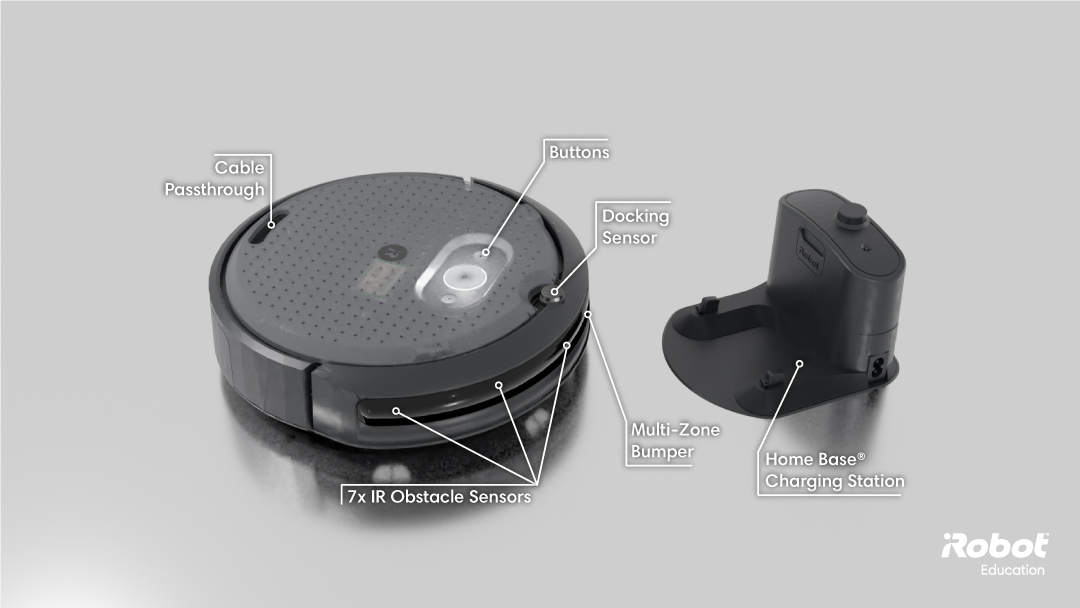
\includegraphics[width=0.8\linewidth]{figures/irobot_create_3}
	\caption[Overview of the iRobot® Create® 3]{Overview of the iRobot® Create® 3}
	\label{fig:irobot_create_3}
\end{figure}

The software ecosystem of the Create 3 base is natively integrated with ROS 2. Sensor telemetry is broadcast continuously via ROS 2 publishers, while internal actuators are controlled, and user commands processed, through standardized ROS 2 subscribers and service servers. Furthermore, the base features pre-programmed autonomous behaviors out of the box, including automated docking, wall-following, and reactive obstacle avoidance. These behaviors can be dynamically triggered, monitored, and adjusted utilizing ROS 2 actions and parameters.

The user interface on the top surface of the base consists of three physical buttons and a centralized LED light ring.

\begin{figure}[!ht]
	\centering
	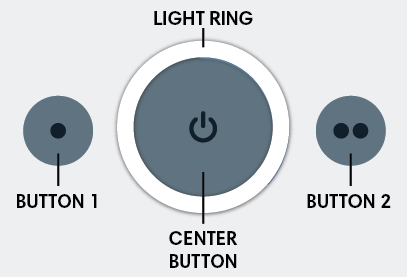
\includegraphics[width=0.7\linewidth]{figures/iRobot_Create_Buttons}
	\caption[Buttons and Light ring on the Base]{Buttons and Light ring configuration on the iRobot Create 3 base and its docking station}
	\label{fig:irobotcreatebuttons}
\end{figure}

The primary center button, marked with a power icon, manages the operational state (power on/off) of the base. The two adjacent, smaller buttons can be mapped to custom user-defined software callbacks. The surrounding LED light ring functions as a visual telemetry indicator, communicating distinct operational states such as active charging, idle standby, system warnings, or critical hardware errors. For exhaustive diagnostics regarding these illumination patterns, the official documentation should be consulted. Additionally, the base includes an autonomous charging dock, allowing the robot to navigate and attach itself independently to replenish its battery.

\newpage

\subsection{Standard Onboard Sensors}
For basic navigation, environmental mapping, and safety enforcement, the TurtleBot 4 relies on a combination of tactile, inertial, and laser-based sensors. The primary payload is the RPLIDAR A1M8 sensor, a 2D LiDAR (Light Detection and Ranging) scanner, mounted on the top deck. This sensor performs continuous 360-degree planar scans of the surrounding environment, generating precise distance measurements that are highly critical for Simultaneous Localization and Mapping (SLAM) and real-time obstacle avoidance.

\begin{figure}[!ht]
	\centering
	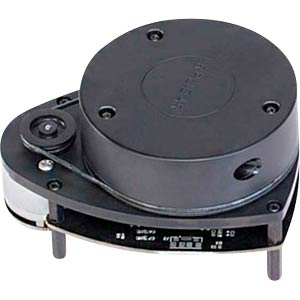
\includegraphics[width=0.5\linewidth]{figures/RPLIDAR_A1M8_sensor.png}
	\caption[RPLIDAR A1M8 LiDAR scanner]{RPLIDAR A1M8 360° Laser Scanner}
	\label{fig:lidar_sensor}
\end{figure}

Odometry tracking is achieved through high-resolution optical wheel encoders working in tandem with an Inertial Measurement Unit (IMU). The wheel encoders measure the exact rotations of the drive wheels to calculate the robot's relative position and velocity over time. The IMU supplements this data by measuring angular velocity and linear acceleration, improving orientation tracking. To ensure operational safety, the front of the iRobot Create 3 base is equipped with a mechanical bumper sensor. This tactile sensor serves as a physical fail-safe; upon physical contact with an object, it instantly triggers a safety interrupt via ROS 2 to halt the actuators, preventing potential damage from obstacles missed by the primary rangefinders.

\subsection{The Luxonis OAK-D Pro Spatial Camera}
For advanced computer vision perception, the TurtleBot 4 is equipped with a Luxonis OAK-D Pro hardware camera module. Structurally, the OAK-D Pro is designed as an all-in-one spatial AI camera platform featuring an onboard Visual Processing Unit (VPU). While this built-in architecture is theoretically capable of executing deep learning neural networks directly on the edge to offload processing tasks from a host system, utilizing the internal VPU for real-time inference was out of scope due to the development timeline constraints of this project.

\begin{figure}[!ht]
	\centering
	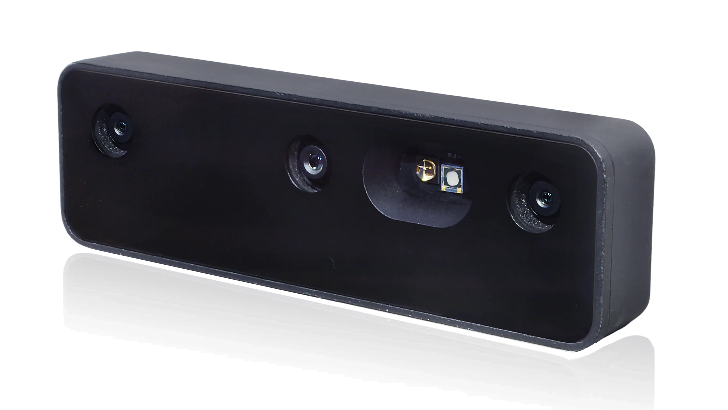
\includegraphics[width=0.6\linewidth]{figures/oakd_pro_camera.png}
	\caption[Luxonis OAK-D Pro Camera]{The Luxonis OAK-D Pro spatial depth camera mounted on the platform.}
	\label{fig:oakd_camera}
\end{figure}

Instead of leveraging the camera's local edge-computing unit, this thesis utilizes the platform as a highly synchronized, raw spatial sensor array. The camera system features a trinocular configuration to gather comprehensive environmental data. It combines two global-shutter monochrome cameras to calculate stereo depth perception with a centralized high-resolution RGB color camera optimized for feature tracking and object classification. 

In the physical hardware configuration of the TurtleBot 4, these heterogeneous image matrices — specifically the synchronized color and stereo depth data streams — are transmitted natively via a physical USB 3.0 interface directly to the onboard Raspberry Pi 4 processing unit. This high-bandwidth connection ensures that the raw sensory data is delivered to the robot's local computing layer with minimal hardware latency. Additionally, the camera features an integrated infrared illumination system, incorporating a dot projector and a flood LED. This configuration enables reliable depth sensing and surface tracking capabilities even in low-light or zero-light laboratory environments, providing a robust stream of spatial information to the robot's primary interface.


\section{ROS2} % ----------------------------------------------------------------
The Robot Operating System (ROS) is a comprehensive set of open-source software libraries and tools designed to facilitate the development of applications for robotic systems. It includes a wide variety of drivers for state-of-the-art algorithms, graphical user interface (GUI) development tools, and extensive resources suitable for any type of robotics project. 

\begin{figure}[!ht]
	\centering
	
\includegraphics[width=0.6\linewidth]{figures/Ros_logo.png}
	\caption[ROS 2 Logo]{ROS 2 Logo}
	\label{fig:ros2}
\end{figure}

Fundamentally, ROS operates as the architectural glue of the entire robotic system. Instead of a monolithic software structure, the developer implements modular components known as nodes to add specific functionalities or support for particular hardware. These nodes communicate with one another asynchronously or synchronously through dedicated mechanisms: topics, services, or actions. Because the communication messages within ROS are strictly standardized, the framework is inherently language-agnostic. Nodes can be developed in different programming languages, provided their inputs and outputs comply with the defined message structures. Consequently, a developer might implement a low-level motor driver in C++ to achieve optimal hardware performance, while simultaneously utilizing Python for high-level image recognition programs or neural networks.

While the framework is commonly referred to simply as ROS, there are actually two distinct generations, known as ROS1 and ROS2 respectively. The first version, ROS1, entered development in 2007 by a company called Willow Garage, originating from a university project at Stanford University. Its first official release was published in March 2010. While this version proved highly successful by introducing features such as a peer-to-peer architecture, computational modularity, and widespread code reusability, it possessed inherent limitations. These included a single point of failure within its centralized ROS Master system, a lack of deterministic real-time support, poor Wi-Fi integration, and no native support for multi-robot setups.

To address these commercial and architectural limitations, the development of ROS2 began in 2014. With its first official alpha release in 2015, a fundamentally redesigned iteration of the framework was introduced. These improvements replaced the legacy ROS Master with an industry-standard Data Distribution Service (DDS) middleware, successfully eliminating the single point of failure. Furthermore, ROS2 introduced native support for real-time execution, robust multi-robot communication, and Quality of Service (QoS) profiles. The latter is highly critical for high-bandwidth data management, such as handling live video streams. Ultimately, these advancements significantly streamlined industrial-grade deployment.
 


\section{YOLO} % -------------------------------------------------------------

The computer vision framework selected for the practical implementation of this thesis is YOLO (an acronym for "You Only Look Once"), specifically the modern iterations maintained by the company Ultralytics. Originally introduced by Joseph Redmon et al. in 2015, the YOLO architecture revolutionized the field of computer vision. Unlike traditional regional-based convolutional neural networks (R-CNNs) that require a two-stage process for region proposal and classification, YOLO frames object detection as a single regression problem. By processing the entire image through a single neural network in a single forward pass, it achieves exceptional inference speeds, making it the premier choice for real-time robotic vision applications.

\begin{figure}[!ht]
	\centering
	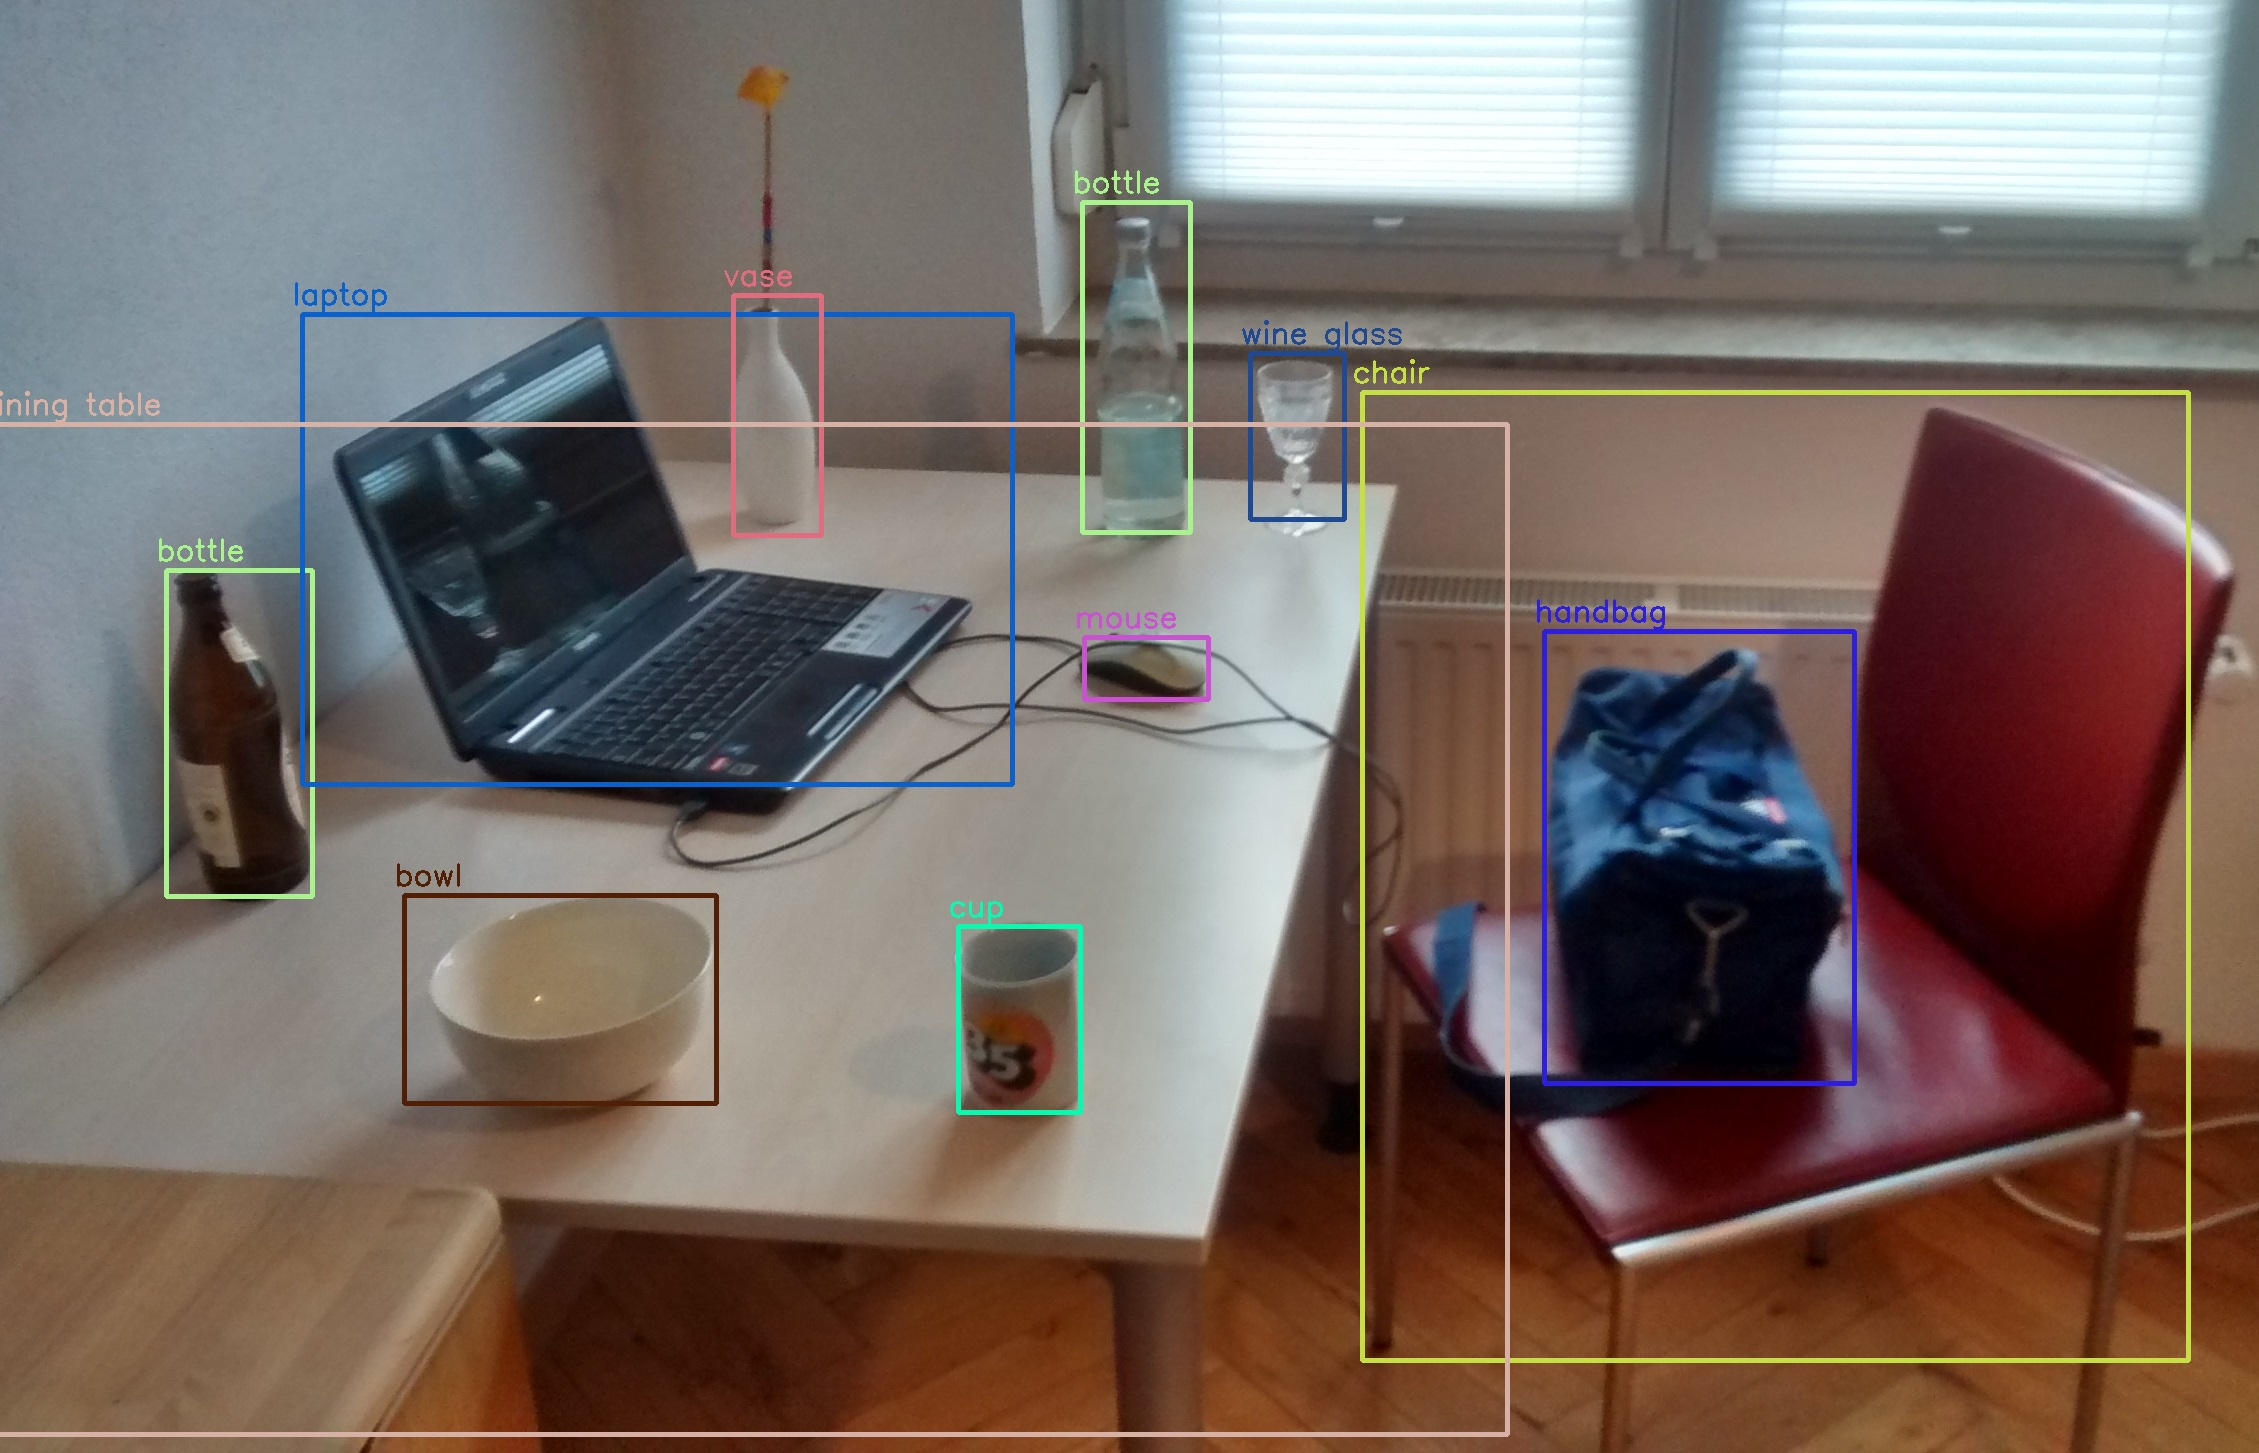
\includegraphics[width=0.6\linewidth]{figures/YOLO_detecting_objects.png}
	\caption[YOLO detecting Objects]{YOLO detecting Objects with the COCO dataset}
	\label{fig:yolo}
\end{figure}

In modern robotics pipelines, Ultralytics' deployment of YOLO has become the industry standard due to its balance between computational efficiency and high precision. The framework provides robust pretrained models that have been optimized using benchmarks trained on millions of labeled images, such as the COCO (Common Objects in Context) dataset. For rapid prototyping and seamless software integration, it features a native Python module. Furthermore, the architecture is highly scalable, offering various model scales ranging from "nano" ($n$) for resource-constrained edge devices like the Raspberry Pi, up to "extra-large" ($x$) for high-performance workstation GPUs. 

Beyond standard object detection (generating 2D bounding boxes), modern versions of YOLO have evolved into comprehensive multi-task vision frameworks. They natively support instance segmentation (pixel-level masking), object tracking across sequential video frames, and pose estimation (keypoint detection). This versatility allows the robotic system to not only identify and locate obstacles or targets but also to understand their orientation, motion vectors, and precise geometry within the environment.

	\chapter{State of the Art}
While the previous chapter established the theoretical foundations of the utilized frameworks and hardware platforms, this chapter examines the current state of research and technological developments relevant to this thesis. Implementing a robust person-following behavior on a mobile robot requires a synthesis of various disciplines. Therefore, the following sections review recent advancements in mobile robotic computer vision, analyze existing methodologies for real-time person detection, evaluate algorithmic strategies for robotic target-following, and discuss current ROS-based solutions within the academic and industrial communities.

\section{Computer Vision in Mobile Robotics}
The integration of computer vision (CV) has fundamentally transformed the paradigm of mobile robot navigation. Historically, autonomous mobile robots (AMRs) relied primarily on active distance sensors, such as ultrasonic rangefinders or planar 2D LiDAR scanners, to map environments and avoid collisions. While highly effective for geometric obstacle detection, these sensors lack semantic understanding; they cannot differentiate between a static wall and a dynamic human agent. To overcome these limitations, vision-based perception has emerged as a cornerstone of intelligent robotics, serving as the primary source for comprehensive scene understanding.

Over the past two decades, the application of computer vision in mobile robotics has evolved through distinct technological phases. Early implementations utilized classical feature-extraction techniques — such as optical flow, edge detectors, and scale-invariant feature transforms (SIFT) — to achieve basic localization and visual odometry. However, these traditional algorithms often exhibited poor robustness when subjected to dynamic illumination changes or unstructured environments. The field experienced a significant shift with the commercialization of RGB-Depth (RGB-D) sensors, which allowed robotic architectures to seamlessly fuse high-resolution color frames with spatial point-cloud data in real time. 

Today, the state of the art in mobile robotic vision is heavily dominated by deep learning frameworks and Spatial AI. Modern robotic systems utilize Convolutional Neural Networks (CNNs) and Vision Transformers running directly on embedded edge-computing hardware. This architecture enables mobile platforms to perform low-latency semantic segmentation, object detection, and behavioral prediction. By leveraging vision intelligence, contemporary robots can interpret complex spatial relationships and contextual cues, establishing the technological baseline required for complex human-robot interaction (HRI) tasks, such as autonomous person following.

\section{Person Detection Methods} %{TODO überarbeitn}
Robust human detection is a critical prerequisite for successful human-robot co-existence and interaction. Within the domain of computer vision, algorithms designed to isolate and identify human targets have progressed from rigid hand-crafted feature extractors to highly adaptable deep learning architectures. Understanding this evolution is essential for evaluating the performance tradeoffs regarding accuracy and computational latency in real-time robotic frameworks.

Historically, classical pedestrian detection relied heavily on the combination of Histogram of Oriented Gradients (HOG) and Support Vector Machines (SVM). Introduced by Dalal and Triggs, this methodology utilizes local gradient directions to capture the characteristic silhouette of the human body. While computationally lightweight compared to modern neural networks, hand-crafted features suffer from severe limitations in dynamic environments. They exhibit poor resilience against illumination variances, scale fluctuations, and structural occlusions—such as a robot viewing a person partially hidden behind office furniture. Similarly, early cascade classifiers (e.g., the Viola-Jones framework) proved highly efficient for facial detection but lacked the required versatility to track full-body movements from a moving robotic platform.

The emergence of Deep Convolutional Neural Networks (CNNs) fundamentally shifted the state of the art by replacing hand-crafted algorithms with automated feature learning. Early deep-learning approaches utilized two-stage detectors like Faster R-CNN, which first extract regions of interest and subsequently classify them. Although highly accurate, the significant computational overhead of two-stage pipelines introduces latency, making them impractical for closed-loop robotic control where immediate sensor feedback is mandatory. 

To bridge this gap, modern mobile robotics heavily utilizes one-stage detectors, primarily the You Only Look Once (YOLO) framework. By formulating detection as a single regression problem, YOLO predicts bounding boxes and class probabilities directly from full image frames in a single forward pass. This architectural efficiency enables real-time inference speeds exceeding standard camera frame rates. Furthermore, modern iterations of these deep networks transcend basic bounding-box generation by incorporating multi-task learning, such as simultaneous object tracking and pose estimation. Consequently, modern person detection methods not only confirm the presence of a human target but also provide structural data regarding orientation and posture, establishing a robust foundation for active target-following behaviors.


\section{Person Following Approaches}
Once a human target has been successfully detected and isolated within the perception pipeline, the robotic system must translate this spatial data into continuous, safe, and reliable locomotive commands. Strategies for executing a person-following behavior typically fall into two major paradigms: purely reactive geometric control and comprehensive path-planning-based navigation. 

Reactive approaches represent the traditional baseline for target tracking. These methods generally rely on geometric relationships derived from camera coordinate frames or LiDAR clusters to maintain a fixed relative distance and orientation to the target. Control structures often utilize classical Proportional-Integral-Derivative (PID) loops or velocity-vector mapping to continuously adjust the robot’s linear and angular speeds. For example, the control loop attempts to minimize the error between the current target distance and a predefined safe tracking distance (e.g., 1.5 meters), while simultaneously centering the target within the robot's field of view. While reactive algorithms offer exceptionally low computational latency and immediate feedback responses, they possess a critical flaw: environmental blindness. Because reactive controllers map velocity vectors directly to the target without evaluating global spatial structures, the platform is prone to clipping corners or colliding with intervening obstacles in cluttered indoor environments.

To address the limitations of reactive tracking, modern research heavily focuses on path-planning-based navigation approaches. Instead of treating target tracking as a direct line-of-sight vector problem, these methods integrate the detected human coordinates dynamically into the robot's navigation stack—such as the ROS 2 Navigation (Nav2) ecosystem. The human target is defined as a continuously updating moving goal within a local costmap. Local path planners, utilizing algorithms like the Dynamic Window Approach (DWA) or Timed Elastic Band (TEB), then calculate kinematically feasible trajectories. This architecture ensures that the robot actively follows the user while simultaneously calculating smooth trajectories to detour around obstacles, walls, or other dynamic agents. Although navigation-based frameworks exhibit higher computational overhead and require robust real-time localization, they provide the operational safety and reliability necessary for real-world deployment in human-populated environments.


\section{Existing ROS-based Solutions}
Within the open-source robotics community, numerous packages have been developed to achieve target tracking and human-following behaviors. Analyzing these existing implementations is crucial to identify architectural limitations and highlight the specific engineering contributions of this thesis within the ROS 2 ecosystem.

In the legacy ROS 1 paradigm, foundational packages such as \texttt{turtlebot\_follower} or various laser-based tracking nodes established early benchmarks. These implementations primarily relied on geometric clustering of 2D LiDAR data to isolate human legs, or utilized basic depth thresholding from early RGB-D sensors to track the closest moving entity. However, these classical solutions suffered from significant reliability issues; they lacked semantic awareness, making them highly susceptible to target-loss errors whenever the user walked near static obstacles or when another human crossed the robot's line of sight.

With the industry migration to ROS 2, contemporary solutions have increasingly integrated deep learning inference nodes with the advanced Navigation 2 (\texttt{Nav2}) stack. Community-driven packages frequently leverage standard ROS 2 wrappers for deep learning frameworks, such as OpenCV or specialized AI toolkits, to publish bounding boxes as localized spatial goals. Despite their improved tracking robustness, a critical challenge remains regarding hardware deployment on mobile platforms. Standard ROS 2 vision pipelines often demand substantial computational overhead. Running state-of-the-art neural networks directly on resource-constrained central processing units—such as the TurtleBot 4’s built-in Raspberry Pi 4—frequently results in severe frame-rate drops and operational latency, which compromises the real-time responsiveness of the robot's control loop. To bypass this bottleneck, many existing setups require offloading the AI inference to an external, high-performance workstation or hardware.

%This thesis addresses these architectural limitations by proposing a distributed, network-decentralized ROS 2 pipeline. While advanced spatial AI sensors like the Luxonis OAK-D Pro feature an integrated Visual Processing Unit (VPU) designed to offload deep learning inference directly to the edge, exploring this specialized hardware integration was constrained by the development timeline of this project. Instead, this research demonstrates a robust alternative approach by offloading the entire computational burden—including high-level YOLO inference and spatial localization—to an external workstation equipped with a high-performance graphics card. Linked seamlessly via CycloneDDS, this architecture completely frees the central Single-Board Computer from vision-related tasks. It bridges the gap between high-precision deep learning perception and standalone robotic navigation, establishing a highly responsive, low-latency person-following framework tailored for resource-constrained mobile platforms


	\chapter{Methodology}
This chapter delineates the methodological framework and engineering design choices utilized to implement the real-time person-following system. It translates the theoretical foundations and state-of-the-art concepts into a concrete architectural blueprint. The following sections outline the precise system requirements, detail the decentralized software-hardware architecture, and explain the algorithmic pipelines responsible for deep-learning-based perception, spatial localization, and robotic motion control.

\section{System Requirements}
To ensure the successful development and deployment of the person-following robot, a rigorous set of system requirements was defined. These criteria are categorized into functional requirements (FR), which dictate the core capabilities of the platform, and non-functional requirements (NFR), which establish the operational constraints and performance benchmarks.

\subsection{Functional Requirements}
\begin{itemize}
	\item \textbf{FR-1: Automated Human Detection:} The system must autonomously identify a human target within the camera's field of view utilizing deep learning object detection models.
	\item \textbf{FR-2: Real-Time Spatial Localization:} The robot must continuously calculate the relative 3D spatial coordinates (X, Y, Z) of the detected person using synchronized depth sensor data.
	\item \textbf{FR-3: Active Target Tracking:} The locomotive base must dynamically adjust its linear and angular velocities to follow the designated human target at a safe distance.
	\item \textbf{FR-4: Integrated Safety Interrupts:} The platform must process physical bumper collisions and emergency stop triggers to halt the actuators instantly, prioritizing user safety.
\end{itemize}

\subsection{Non-Functional Requirements}
\begin{itemize}
	\item \textbf{NFR-1: Low Latency Inference:} The entire perception-to-actuation pipeline must operate with minimal latency, targetting a real-time frame rate of at least 15 to 30 frames per second (FPS) on the edge device.
	\item \textbf{NFR-2: Computational Efficiency:} High-level deep learning tasks must not overload the central processing unit (Raspberry Pi 4), ensuring that critical robotic navigation services remain stable.
	\item \textbf{NFR-3: Modular Software Architecture:} The software components must be decoupled into independent ROS 2 nodes to ensure scalability, ease of debugging, and maintainability.
\end{itemize}

\section{Overall System Architecture}
The architectural design of the proposed system utilizes a distributed offloading paradigm due to the heavy computational demands of deep learning inference. Initial testing revealed that the onboard Raspberry Pi 4 Single-Board Computer (SBC) lacked the processing capabilities required to run the YOLO object detection pipeline at a responsive real-time frame rate. While the Luxonis OAK-D Pro camera features an integrated Visual Processing Unit (VPU) capable of edge computing, utilizing this onboard hardware was out of scope for the timeline of this thesis. 

Consequently, the physical framework is divided into a dedicated external computing unit and the mobile robot platform. The raw sensory data from the OAK-D Pro camera is passed directly through the Raspberry Pi 4 without local processing and transmitted over a local wireless network to an external workstation (laptop). This workstation serves as the primary processing hub, executing the high-level computer vision models, spatial localization, and state machine transitions. Communication and data synchronization between the external laptop and the TurtleBot 4 base are managed natively via the Eclipse CycloneDDS middleware, ensuring low-latency transport of control commands back to the iRobot Create 3 base actuators.


\section{Software Design}
The software architecture is designed around the principles of modularity and asynchronous communication inherent to ROS 2. Rather than relying on a single, monolithic executable, the system is divided into specialized, decoupled software components known as nodes. 

Communication between these nodes is achieved through standardized ROS 2 interfaces, specifically utilizing topics for high-frequency telemetry and actions for long-running, interruptible behaviors. To prevent data corruption or race conditions, the nodes utilize a language-agnostic data layout. This modular software design allows the system to remain highly robust; for instance, if the high-level perception pipeline experiences a momentary delay, the lower-level safety layers on the mobile base can still act independently to prevent collisions.

\subsection{Detection Pipeline}
The detection pipeline is responsible for extracting semantic meaning from raw environmental inputs. Instead of processing data locally on the camera hardware, it utilizes the YOLO architecture executing directly on the external laptop workstation. The raw, high-resolution RGB image stream captured by the OAK-D Pro sensor array is transmitted over the network and continuously downscaled on the host machine to match the specific input matrix dimensions required by the neural network.

\begin{figure}[!ht]
	\centering
	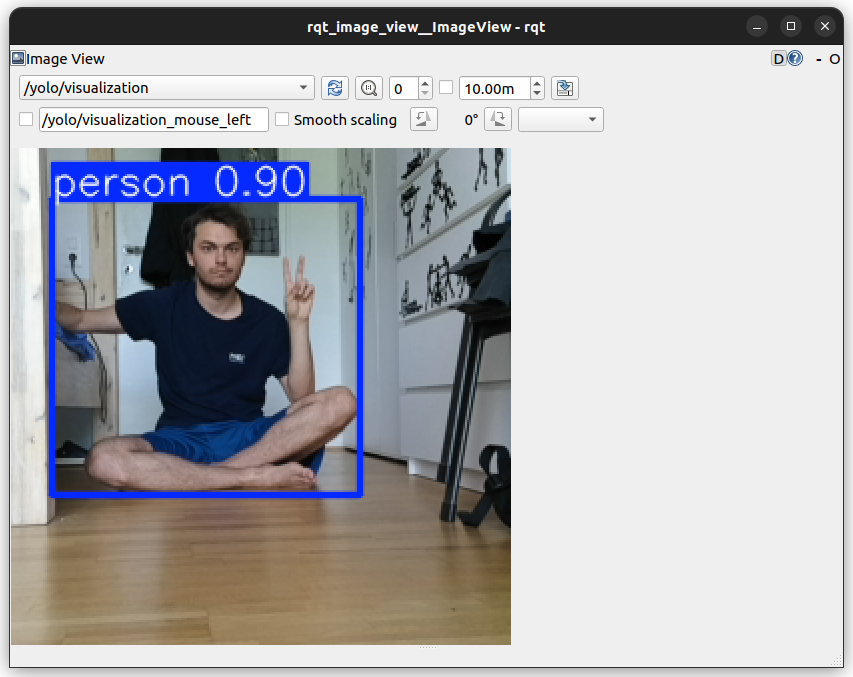
\includegraphics[width=0.8\linewidth]{figures/det_pipeline.png}
	\caption[Detection Pipeline]{Detection pipeline detecting a human}
	\label{fig:det_pipeline}
\end{figure}

The forward pass of the model, computed entirely by the workstation's graphics processor, generates boundary bounding boxes, class labels, and confidence scores for all detected entities within the frame. A specialized software filter is subsequently applied within the custom ROS 2 node to discard all classes except the "person" label. To minimize false positives and ensure stable tracking, a confidence threshold of $\tau \ge 0.8$ is enforced. The final output of this pipeline is a filtered 2D bounding box representing the precise horizontal and vertical pixel coordinates of the human target within the image plane, which is then made available for spatial localization.

\section{Object Localization}
Once the 2D bounding box of the human target is established, the object localization module maps these pixel coordinates into a 3D spatial coordinate frame relative to the robot. This is achieved by fusing the 2D vision data with the synchronized stereo depth map provided by the camera's global-shutter monochrome sensors.

\begin{figure}[!ht]
	\centering
	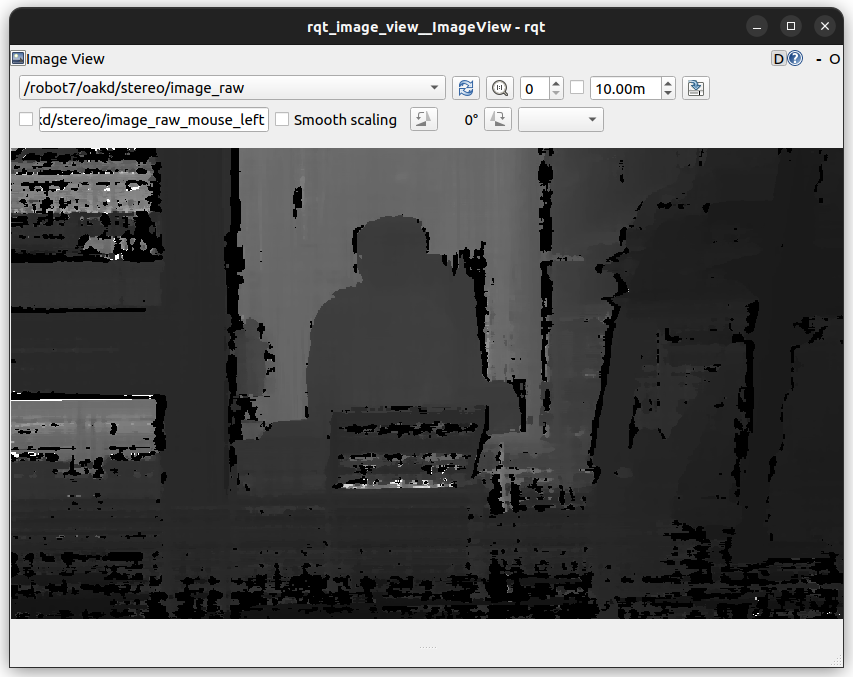
\includegraphics[width=0.8\linewidth]{figures/depth_image.png}
	\caption[Stereo depth image]{Stereo depth image}
	\label{fig:stereo_image}
\end{figure}

The algorithm calculates the region of interest (ROI) on the depth map that corresponds to the center of the 2D bounding box. By extracting the median depth value within this spatial patch, the system determines the absolute Euclidean distance ($Z$) along the camera's optical axis. Using the camera's intrinsic calibration parameters—specifically the focal length ($f_x, f_y$) and the optical center ($c_x, c_y$)—the system applies pixel-to-3D back-projection. This mathematical transformation yields the exact spatial coordinates $(X, Y, Z)$ of the target in meters, which are then continuously published as a standardized coordinate transform (TF2) tree within ROS 2.

\section{Person Following Strategy}
The locomotive strategy of the robot is governed by a Finite State Machine (FSM). This architectural choice ensures predictable and robust transitions between different operational phases based on the tracking status of the target. The logical flow and transition conditions between the individual states are illustrated in Figure~\ref{fig:fsm_transitions}.

\begin{figure}[!ht]
	\centering
	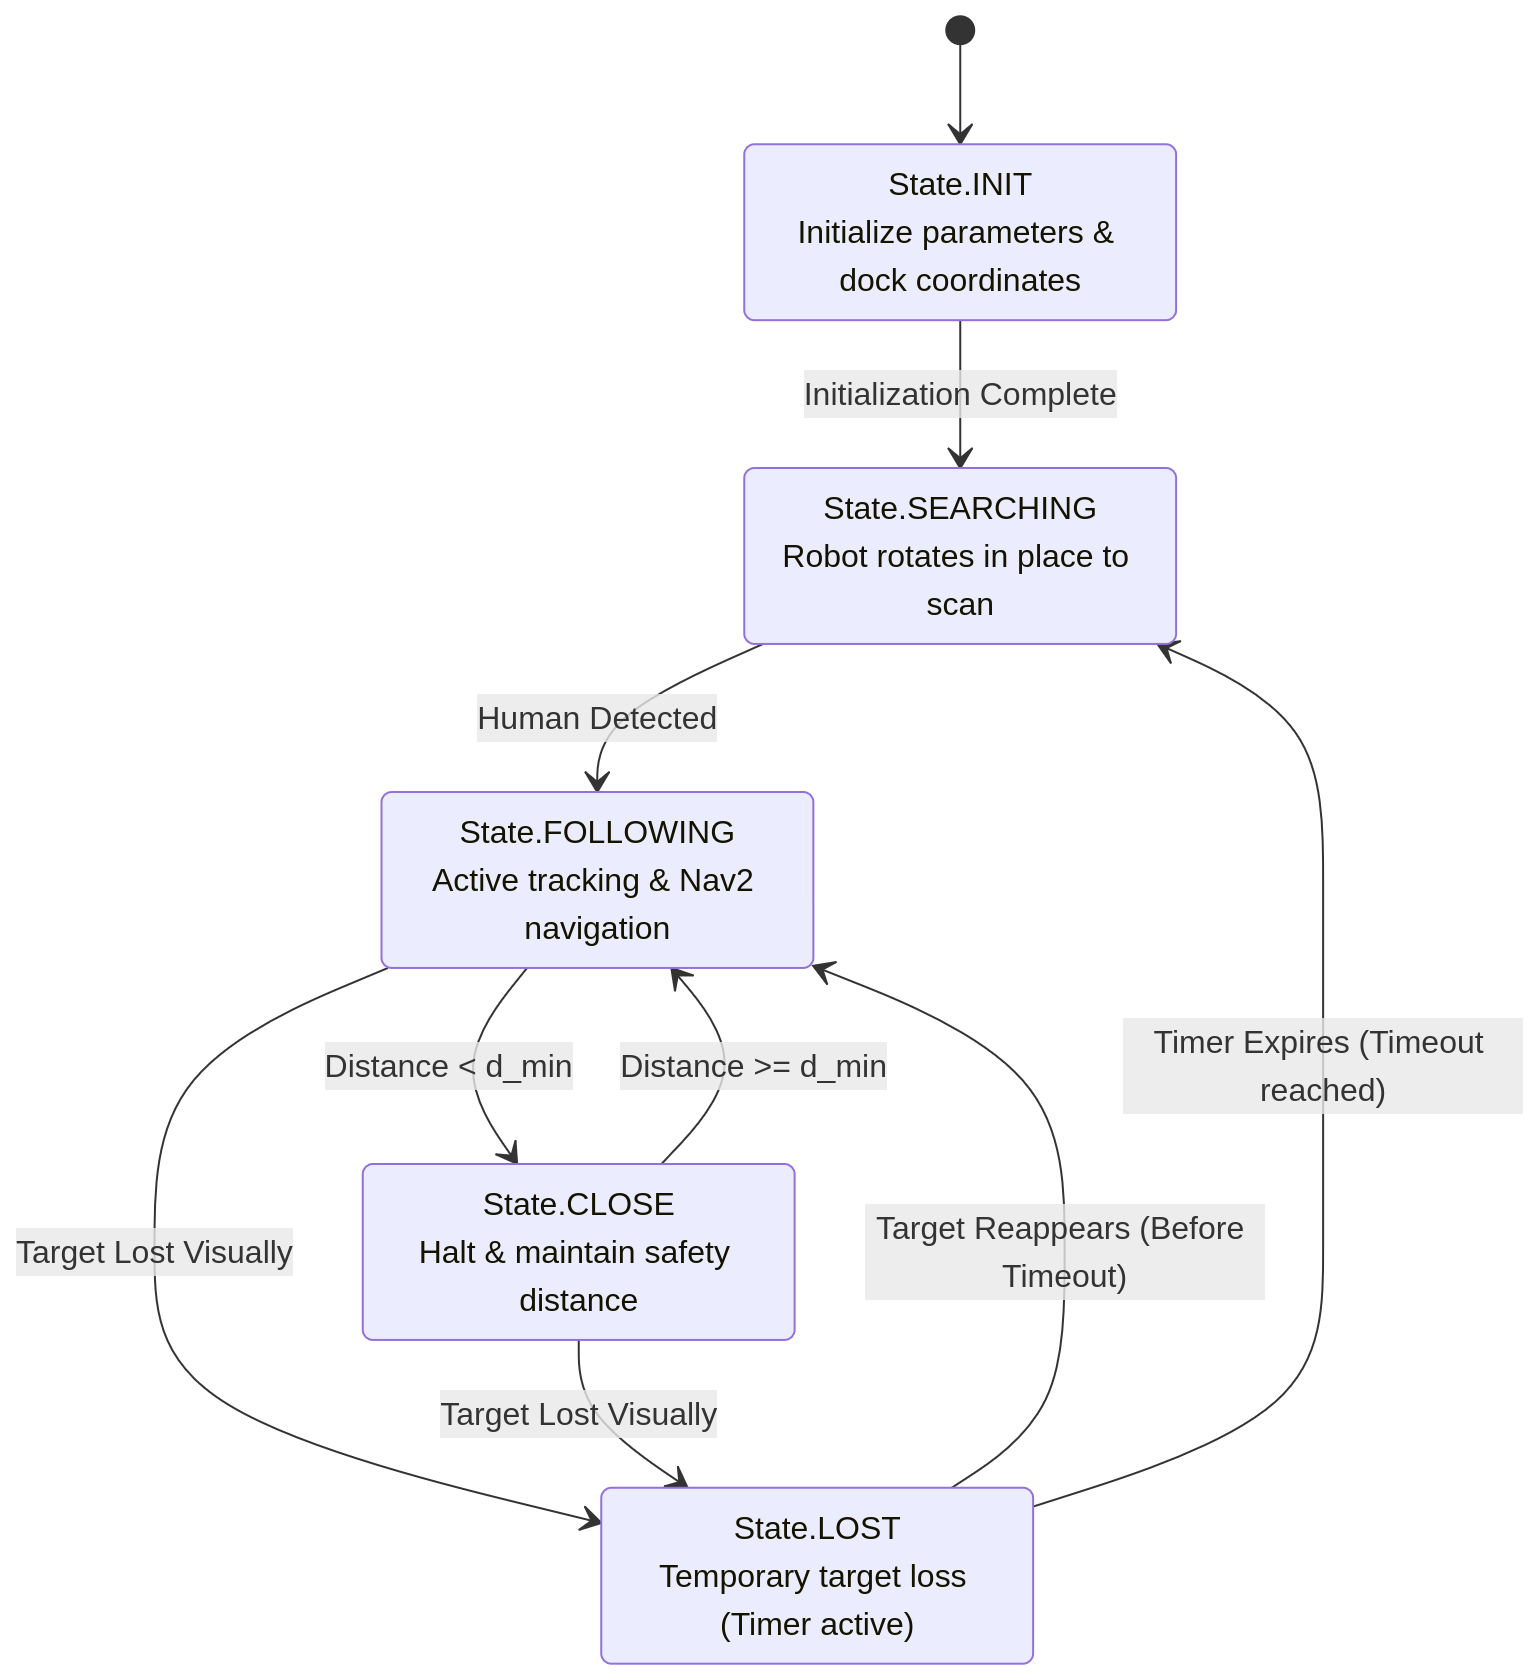
\includegraphics[width=0.8\linewidth]{figures/state_machine.png}
	\caption[Finite State Machine Transition Diagram]{State transition diagram of the centralized controller, highlighting the operational logic from initialization to target loss handling.}
	\label{fig:fsm_transitions}
\end{figure}

\newpage

The FSM consists of five distinct states:

\begin{itemize}
	\item \textbf{\texttt{State.INIT}:} The initialization phase where essential baseline parameters and starting conditions are established, such as capturing the robot's initial position while docked at the charging station.
	\item \textbf{\texttt{State.SEARCHING}:} Triggered when no human target is visible. In this state, the robot executes a continuous, controlled rotation in place to scan its surroundings and locate a person.
	\item \textbf{\texttt{State.FOLLOWING}:} The active tracking state. The robot computes the distance and angle to the detected human and follows them smoothly until the target either enters the safety zone or is visually lost.
	\item \textbf{\texttt{State.CLOSE}:} A safety-enforcement state activated when the human target is within close proximity. The TurtleBot 4 stops its translational movement to maintain a strict predefined safety distance from the person.
	\item \textbf{\texttt{State.LOST}:} A temporary transitional state entered immediately when the person disappears from the camera's field of view. A software timer is initiated upon entering this state. If the target reappears within the image frame before the timer expires, the FSM transitions smoothly back to \texttt{State.FOLLOWING}. If the timer running out confirms the target is permanently lost, the robot reverts to \texttt{State.SEARCHING}.
\end{itemize}

	\chapter{Experimental Implementation}
Following the methodological framework outlined in the previous chapter, this section details the concrete experimental implementation of the person-following system. It describes the practical deployment of the software stack, the configuration of the distributed network nodes, and the structural implementation of the control loops. This chapter serves as a comprehensive technical guide, moving from the initial environment setup to the specific programming of the computer vision and navigation nodes.

\section{Development Environment}
To develop and deploy applications within a modern robotics ecosystem, a stable and specialized development environment is paramount. While recent iterations of the Robot Operating System (ROS 2) offer limited compatibility with Windows architectures, the framework is natively designed for and best optimized on Linux distributions. For the implementation of this thesis, ROS 2 Humble Hawksbill was deployed on an Ubuntu 22.04 LTS (Jammy Jellyfish) operating system. Because ROS 2 is primarily managed via command-line interface (CLI) terminal inputs, the core framework operates efficiently without demanding specialized external package managers for its basic management.

The software components—comprising both the custom ROS 2 nodes and the high-level YOLO perception models—were implemented using the Python programming language. Python was selected due to its expressive syntax, object-oriented programming (OOP) support, and its extensive ecosystem of data-science libraries, making it an ideal language for rapid software prototyping in research environments. To ensure software stability and prevent dependency conflicts across the system, a Python Virtual Environment (venv) was established. This isolated container allows for the secure installation and version management of required external modules, including the \texttt{ultralytics} suite for machine learning inference and \texttt{opencv-python} for image matrix manipulation, without altering the global system environment.

To maintain historical records of the codebase, track changes, and facilitate structured development, Git was utilized as the primary version control system in combination with GitHub as the cloud-based repository hosting service. This setup ensured a reliable backup of the source code and allowed for systematic debugging by enabling rollbacks to previous stable software states. For the actual code writing, Visual Studio Code (VSCode) was chosen as the Integrated Development Environment (IDE). 

Managing the distributed architecture required seamless remote access to the TurtleBot 4's onboard Single-Board Computer (SBC). While standard remote administration is achievable through native Secure Shell (SSH) terminal commands, a more integrated approach was chosen by leveraging the VSCode Remote - SSH extension. This extension allows the developer to connect the local IDE directly to the robot's filesystem over the wireless network, streamline real-time code editing, and interact with the robot's environment through a single, unified development interface.

Finally, all custom-developed nodes and configurations described in the subsequent sections of this chapter were organized into a single, dedicated ROS 2 package named \texttt{yolobot}. In the ROS 2 ecosystem, a package serves as the fundamental organizational unit used to bundle software, custom message definitions, launch files, and dependency manifests. By encapsulating the entire implementation within the \texttt{yolobot} package, the project maintains a high degree of modularity, ensuring that the developed person-following pipeline can be easily compiled, transferred, and reused on other ROS 2-compatible robotic systems.

\section{YOLO Detection Node}
The core perception capabilities of the software stack are encapsulated within the \texttt{yolo\_detect} node. Developed as the initial component of the \texttt{yolobot} package, this node is responsible for executing real-time object detection and transforming raw sensory data into structured semantic information. 

Architectural interactions and data flows of this node within the ROS 2 ecosystem are illustrated in Figure~\ref{fig:yolo_node_graph}.

\begin{figure}[!ht]
	\centering
	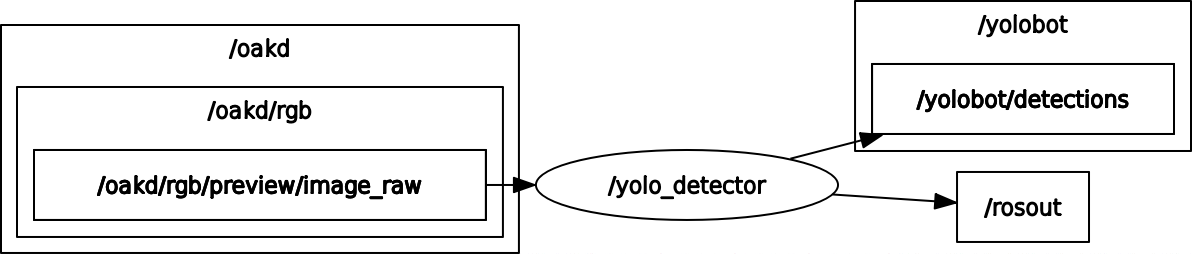
\includegraphics[width=0.8\linewidth]{figures/yolo_detector.png}
	\caption[ROS 2 Node Graph for yolo\_detect]{Computation graph displaying the input image subscription and output bounding box publishers for the yolo\_detector node.}
	\label{fig:yolo_node_graph}
\end{figure}

The functional mechanism of the node relies on an asynchronous callback pipeline. The node subscribes to the raw image telemetry broadcast by the spatial camera on the \texttt{robot7/oakd/rgb\newline/preview/image\_raw} topic. Upon receiving a standardized ROS \texttt{sensor\_msgs/msg/Image} message, the node utilizes the \texttt{cv\_bridge} library to convert the image matrix into a BGR format compatible with OpenCV.

The converted frame is subsequently processed by the YOLO object detection model. To optimize performance and ensure deterministic behavior tailored to this application, the model is configured with a strict confidence threshold ($\tau = 0.8$) and filtered to exclusively retain class ID $0$, which corresponds to the "person" label within the COCO dataset. The model extracts the resulting two-dimensional coordinates of the bounding boxes, populates a standardized \texttt{vision\_msgs/msg/Detection2DArray} message, and publishes the localized metadata to the \texttt{/yolo/detections} topic.

In the early stages of development, the vision pipeline was split across three distinct standalone nodes to decouple verification from data transmission: \texttt{yolo\_basic} managed standard terminal output logs, \texttt{yolo\_viz} published annotated image streams for visual validation, and \texttt{yolo\_detect} handled array publishing. To eliminate software redundancies and reduce network overhead, these variations were refactored into a single, unified node. The core image processing routine is detailed in Listing~\ref{lst:yolo_process}.

\lstinputlisting[linerange={113-134},language=Python,caption={Core image processing and bounding box extraction callback within the unified node.},label={lst:yolo_process}]{codes/yolo_detect.py}

The operational behavior of this consolidated node can be dynamically adjusted at runtime utilizing the native ROS 2 parameter server. By toggling the \texttt{enable\_basic} and \texttt{enable\_viz} parameters respectively, the user can conditionally activate localized logging or video visualization features. The structural implementations of these optional sub-modules are presented in Listings~\ref{lst:yolo_basic} and \ref{lst:yolo_viz}.

\lstinputlisting[linerange={195-204},language=Python,caption={Optional logging logic controlled via the enable\_basic parameter.},label={lst:yolo_basic}]{codes/yolo_detect.py}

\lstinputlisting[linerange={206-221},language=Python,caption={Optional stream annotation and visualization publisher controlled via the enable\_viz parameter.},label={lst:yolo_viz}]{codes/yolo_detect.py}

To ensure seamless deployment across different host machines without requiring absolute file path definitions, the node is engineered to resolve its asset paths dynamically relative to the ROS 2 workspace workspace structure. The neural network weights (\texttt{.pt} files) are allocated a dedicated directory within the share space of the package. During the node's instantiation phase, the path is resolved programmatically, allowing the framework to securely load the model file regardless of the global deployment environment, as demonstrated in Listing ~\ref{lst:yolo_path}.

\lstinputlisting[linerange={45-50},language=Python,caption={Dynamic resolution of the internal package path for model instantiation.},label={lst:yolo_path}]{codes/yolo_detect.py}

\section{Object Localization Node}
The \texttt{object\_locator} node functions as a critical translation and data-fusion layer between the high-level perception pipeline (\texttt{yolo\_detect}) and the downstream navigation state machine. The primary responsibility of this node is to project two-dimensional bounding box coordinates into accurate three-dimensional spatial coordinates relative to the robot's reference frame.

The architectural interactions, incoming topic subscriptions, and outgoing data streams for this node are visualized in Figure~\ref{fig:locator_node_graph}.

\begin{figure}[!ht]
\centering
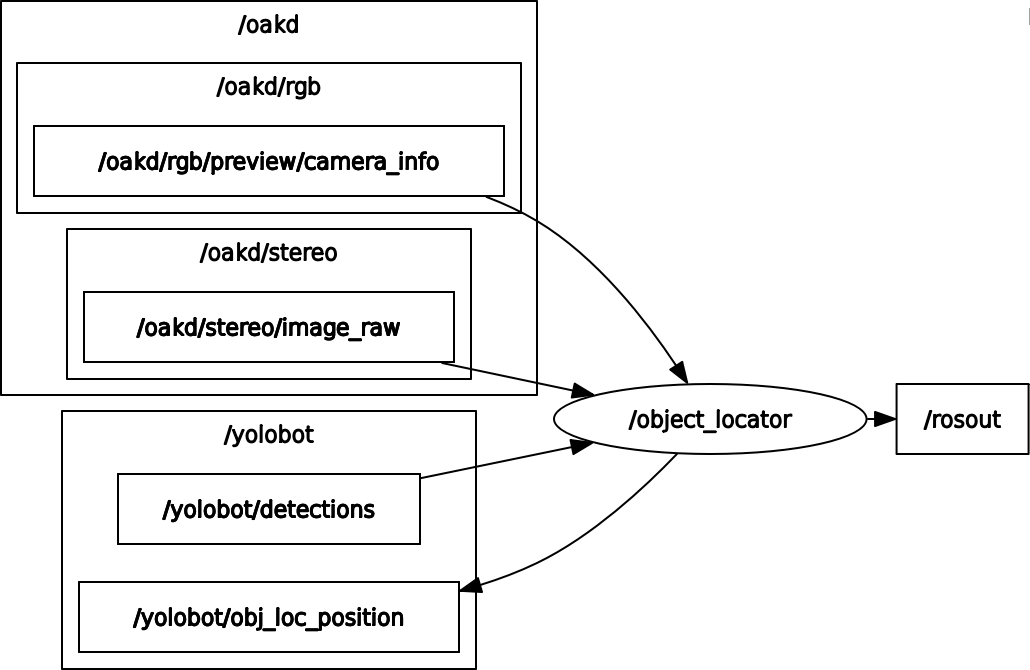
\includegraphics[width=0.8\linewidth]{figures/object_locator.png}
\caption[ROS 2 Node Graph for object\_locator]{Computation graph illustrating the input subscriptions from the YOLO detection node and camera topics, alongside the output spatial coordinate publishers.}
\label{fig:locator_node_graph}
\end{figure}

To perform spatial calculations, the node subscribes to a heterogeneous array of four distinct data streams using standardized ROS~2 interfaces:
\begin{itemize}
\item \textbf{YOLO Detections Sub}: Subscribes to the \texttt{/yolo/detections} topic, ingesting messages of type \texttt{vision\_msgs/msg/Detection2DArray} to receive the bounding boxes from the perception pipeline.
\item \textbf{Camera Info Sub}: Subscribes to the \texttt{/robot7/oakd/rgb/preview/camera\_info} topic using the \texttt{sensor\_msgs/msg/CameraInfo} message type to extract lens intrinsic parameters required for spatial back-projection.
\item \textbf{Stereo Depth Sub}: Subscribes to the \texttt{/robot7/oakd/stereo/image\_raw} topic using the \newline \texttt{sensor\_msgs/msg/Image} message type to acquire the structured depth matrices calculated by the camera.
\item \textbf{RGB Image Sub}: Subscribes to the \texttt{/robot7/oakd/rgb/preview/image\_raw} topic, also utilizing the \texttt{sensor\_msgs/msg/Image} type, to capture the live color frames for alignment and visualization.
\end{itemize}

By fusing these internal memory variables via an asynchronous callback scheme, the node calculates the absolute Euclidean distance along the camera’s optical axis. This mathematical transformation yields the exact spatial coordinates $(X, Y, Z)$ of the target in meters, which are then continuously published to the \texttt{/yolo/object\_position} topic as a standardized \texttt{geometry\_msgs/msg/PointStamped} message.

While the primary objective of this thesis is human tracking, the localization pipeline was engineered to be highly modular and object-agnostic. Because the localization logic operates independently of the underlying semantic classification, the system can locate any arbitrary object without modifying the core localization algorithm. The only adaptation required to track different entities would be adjusting the class filtering parameters within the preceding \texttt{yolo\_detect} node. This modular separation of concerns justifies the architectural decision to implement localization as a standalone node. Consequently, the \texttt{object\_locator} can be seamlessly repurposed in future applications to publish spatial coordinates of obstacles for collision avoidance, alternative target-tracking algorithms, or be extended to aggregate multi-camera inputs.

%\lstinputlisting[linerange={1-50},language=Python,caption={Spatial back-projection and depth fusion routine within the object\_locator node.},label={lst:locator_process}]{codes/object_locator.py}

Finally, to streamline real-time validation and debugging during experimental testing, a dedicated ROS~2 parameter named \texttt{visual} was integrated into the node configuration, defaulting to a boolean value of \texttt{False}. When a user explicitly toggles this configuration flag to \texttt{True}, an optional visualization sub-module is triggered. This module spins up an additional publisher targeting the \texttt{/yolo/debug\_image} topic with a \texttt{sensor\_msgs/msg/Image} payload. This debug stream overlays the calculated spatial coordinates, distance metrics, and bounding-box targets directly onto the live color frame for visual verification. %An example layout for this visual validation is reserved in Figure~\ref{fig:locator_debug}.

%\begin{figure}[!ht]
%\centering
% \includegraphics[width=0.7\linewidth]{figures/locator_debug_output}
%\caption[Visual Debug Output of the Object Locator]{Example of the generated debug stream displaying spatial coordinate overlays and distance tracking vectors.}
%\label{fig:locator_debug}
%\end{figure}

%\lstinputlisting[linerange={267-361},language=Python,caption={Conditional debug visualization and image publishing logic.},label={lst:locator_debug_code}]{codes/obj_loc.py}

\section{Navigation Integration}
The actuation and path-planning layers of the proposed system are fully integrated into the ROS 2 Navigation (\texttt{Nav2}) ecosystem. Instead of utilizing direct, reactive velocity commands, the TurtleBot 4 leverages advanced global and local planners to safely navigate through human-populated environments. 

The baseline requirement for this navigation pipeline is a static occupancy grid map of the environment. This map is generated prior to the execution of the person-following tasks by manually driving the platform through the operational space while running a Simultaneous Localization and Mapping (\texttt{SLAM}) toolbox. Once completed, the static map is saved and passed down to the \texttt{Nav2} map server. Within this subsystem, global costmaps handle the overall static environment geometry, while local costmaps continuously integrate sensory updates to adapt to transient changes. By building upon this infrastructure, the robot can compute collision-free trajectories, automatically detouring around walls and furniture while maintaining active path planning toward its target destination.

%The computational data flow and node interactions governing this navigation stack are preserved in Figure~\ref{fig:nav_integration_graph}.

%\begin{figure}[!ht]
%	\centering
%	\includegraphics[width=0.8\linewidth]{figures/}
%	\caption[ROS 2 Node Graph for Nav2 Integration]{Computation graph showing the integration of the static map server, localization nodes, and the Nav2 path planners.}
%	\label{fig:nav_integration_graph}
%\end{figure}

% % NOTE: Outcommented listings to prevent compiler errors. Activate when source files are ready.
% \lstinputlisting[linerange={1-30},language=Python,caption={Configuration and initialization scheme for the Nav2 lifecycle nodes.},label={lst:nav2_init}]{codes/navigation_integration.py}


\section{State Machine Implementation}
The decision-making hierarchy and navigational lifecycle of the robot are controlled by a centralized Finite State Machine (\texttt{FSM}). This software node coordinates the overall system behavior by acting as the main interface between the perception pipeline and the \texttt{Nav2} stack. The computational graph and topic layout for the state machine execution are outlined in Figure~\ref{fig:fsm_node_graph}.

\begin{figure}[!ht]
	\centering
	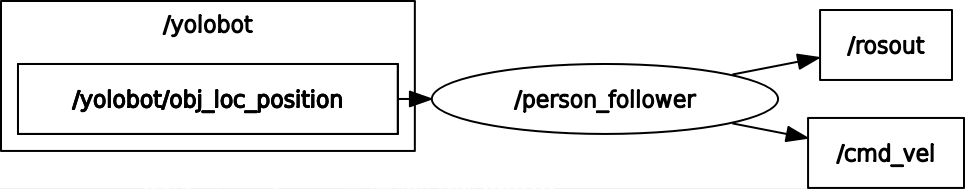
\includegraphics[width=0.8\linewidth]{figures/person_follower.png}
	\caption[ROS 2 Node Graph for the FSM Controller]{Computation graph displaying the transformation of perception topics into Nav2 goal poses controlled via the state machine.}
	\label{fig:fsm_node_graph}
\end{figure}

The state machine node subscribes to the \texttt{/yolo/object\_position} topic to ingest the target's 3D spatial metadata formatted as a \texttt{geometry\_msgs/msg/PointStamped} message. Crucially, because \texttt{Nav2} actions require a definitive target orientation alongside position, the node executes an internal data conversion pipeline. The incoming point data is encapsulated and transformed into a \texttt{geometry\_msgs/msg/PoseStamped} message type, adding default orientation quaternions pointing toward the target. This generated pose is then actively dispatched as a navigational goal to the \texttt{Nav2} action servers.

The operational tracking logic fluidly cycles through five distinct states based on environmental stimuli:
\begin{itemize}
	\item \textbf{\texttt{State.INIT}:} The startup routine responsible for setting baseline software variables and logging initial coordinates, including the robot's physical origin position when docked in its charging dock.
	\item \textbf{\texttt{State.SEARCHING}:} Active when the perception topics yield no detections. The node bypasses the global planner and instructs the base to rotate continuously in place, scanning the environment to discover a person.
	\item \textbf{\texttt{State.FOLLOWING}:} Executed when a valid target is identified. The node continuously intercepts the \texttt{PointStamped} coordinates, transforms them into a \texttt{PoseStamped} format, and forwards these target goals to \texttt{Nav2} to actively navigate toward the moving person.
	\item \textbf{\texttt{State.CLOSE}:} A safety threshold intercept. If the tracking coordinates reveal that the distance to the target falls below a predefined safety margin, the node aborts the current \texttt{Nav2} path execution, halting the TurtleBot 4 to enforce a strict physical buffer zone.
	\item \textbf{\texttt{State.LOST}:} A temporary transitional safety phase triggered upon sudden visual target loss. An internal software timer is immediately spawned. If the human target passes back into the camera's field of view before the timeout expires, the node triggers a smooth transition back into \texttt{State.FOLLOWING}, preventing abrupt stops. If the timer running out confirms a complete target loss, the system reverts to \texttt{State.SEARCHING}.
\end{itemize}

% % NOTE: Outcommented listings to prevent compiler errors. Activate when source files are ready.
% \lstinputlisting[linerange={1-60},language=Python,caption={State machine callback routines, PointStamped-to-PoseStamped conversion, and Nav2 action client dispatch logic.},label={lst:fsm_core}]{codes/state_machine.py}

\section{Testing Procedure}
To evaluate the functional reliability and structural robustness of the integrated software-hardware pipeline, a series of experimental tests was conducted. The primary objective of these procedures was to validate the real-time performance of the detection nodes, the accuracy of the spatial state machine transitions, and the physical safety features of the navigation stack under real-world conditions.

The experimental testing environment was established within a confined indoor space characterized by standard diurnal ambient lighting conditions and unmodified default robotic performance parameters, such as linear and angular velocity limits. Due to its complex spatial geometry and the presence of various arbitrary static obstacles (e.g., household furniture and irregular floor items), this setting provided a highly challenging and realistic proving ground for single-person tracking. This intricate layout allowed for the rigorous evaluation of two critical system capabilities:
\begin{itemize}
	\item \textbf{Dynamic Obstacle Avoidance:} Verifying whether the \texttt{Nav2} local planners could compute collision-free trajectories to bypass tight corners and intervening obstacles while actively pursuing the moving target.
	\item \textbf{Line-of-Sight Occlusion Handling:} Testing the robustness of the \texttt{State.LOST} timer thresholds when the human target was temporarily obscured by spatial architecture or sharp turns.
\end{itemize}

A recognized limitation of this testing procedure was the spatial constraint of the environment. Due to the limited physical dimensions of the room, the maximum operational range and long-distance tracking thresholds of the person-following system could not be fully evaluated. Consequently, comprehensive high-velocity and wide-area benchmarks are reserved for future validation phases.

	\chapter{Results}
This chapter presents the empirical findings and performance metrics gathered during the experimental evaluation of the integrated robotic vision system. To verify the efficacy of the proposed distributed ROS 2 framework, benchmarks were collected across three primary operational axes: the computational efficiency of the perception pipeline, the metric precision of the spatial localization node, and the trajectory reliability of the person-following control loop. The subsequent sections provide a detailed analysis of these quantitative and qualitative results based on the testing procedures established in the previous chapter.

\section{Object Detection Performance}
The performance of the primary perception pipeline closely aligned with the algorithmic expectations of the well-established YOLO framework. However, the practical evaluation highlighted significant hardware-dependent performance variations. Initial implementation attempts focused on executing the object detection models locally on the TurtleBot 4's embedded Raspberry Pi 4 Single-Board Computer. Experimental benchmarks revealed that the onboard ARM-based processor lacked the required computational capacity; even when deploying the highly optimized "nano" ($n$) scale model, the system suffered from critical frame-rate drops and severe latency, rendering closed-loop robotic tracking impossible.

Following the paradigm shift toward a distributed network offloading architecture, the perception workload was transferred to the external workstation. Upon migrating the inference tasks to the workstation's high-performance graphics hardware, the processing capability experienced a substantial upgrade. The system not only achieved fluid real-time frame rates but successfully scaled up to utilize the "extra-large" ($x$) YOLO model configurations. This transition significantly enhanced human feature extraction and classification precision without bottlenecking the robotic middleware.

During continuous tracking sequences under standard ambient lighting, the inference loop operated with high speed and reliability. A minor qualitative edge-case was identified during testing: when the human target was briefly obstructed by tight geometric architecture or household obstacles, the system occasionally registered transient false positives or split detections for a fraction of a second. Aside from these brief latency fluctuations during partial occlusions, the workstation-hosted YOLO pipeline provided a highly stable and dependable semantic stream, establishing a robust foundation for continuous spatial localization.

\section{Localization Accuracy}
The performance of the \texttt{object\_locator} node demonstrated high efficacy in transforming two-dimensional camera bounding boxes and synchronized stereo depth matrices into three-dimensional spatial coordinates. Empirical testing confirmed that the Euclidean distance calculations along the camera's optical axis were highly accurate and remained well within an acceptable operational margin of error for indoor target tracking. 

However, the experimental evaluation revealed a critical architectural challenge regarding real-time data throughput and network latency. Because the localization node simultaneously subscribes to multiple high-bandwidth data streams—including two separate, uncompressed image topics for RGB frames and stereo depth maps—the system is forced to ingest and process a massive volume of data per second. Over continuous operational periods, a noticeable processing lag accumulates within the pipeline, causing the localization coordinates to drift behind the real-time position of the target.

To mitigate this latency, several software optimization strategies were implemented and evaluated:
\begin{itemize}
	\item \textbf{Subscription Management:} Unnecessary or redundant topic subscriptions were programmatically terminated to streamline the node's execution loop.
	\item \textbf{Quality of Service (QoS) Tuning:} The ROS~2 QoS profiles were adjusted to prioritize volatile, best-effort data delivery over historical reliability, allowing the system to drop old frames in favor of the most recent sensor updates.
	\item \textbf{Visualization Deactivation:} Computational overhead was further reduced by disabling all optional image annotation and debug visualization publishers (\texttt{visual = False}).
\end{itemize}

Despite these optimizations, a persistent communication bottleneck remained. Quantitative analysis indicates that the primary constraint is not the CPU processing limits of the workstation, but rather the physical bandwidth limitations of the DDS middleware when transmitting heavy image messages over a wireless network link. The high frequency and sheer size of the arriving image packets saturate the wireless network, introducing transport delays. This transmission lag directly impacts the performance of the downstream \texttt{person\_follower} state machine, as it receives delayed positional updates, thereby challenging the fluid responsiveness of the robot's real-time trajectory control.

\subsection{Person Following Performance}
The empirical evaluation of the centralized Finite State Machine (FSM) demonstrated that after resolving initial configuration challenges, the high-level control logic transitions smoothly and predictably between its five operational states. The logic successfully managed the execution of individual state routines under nominal conditions. However, the practical deployment of the autonomous person-following behavior was heavily impacted by a prominent system bottleneck.

The primary operational constraint stems directly from the previously identified localization latency. Because the 3D coordinate updates arrive at the FSM with a persistent processing lag, the robot's real-time actuation suffers from an algorithmic delay. This latency introduces a severe control loop error during the \texttt{State.SEARCHING} phase. As the TurtleBot~4 executes a continuous rotation in place to scan for a human target, the delayed perception data causes the platform to overshoot the target's actual physical position. By the time the workstation processes the message confirming a human detection, the physical orientation of the robot has already rotated past the camera's field of view. Consequently, this systemic overshoot results in an immediate loss of the target, forcing the FSM back into the searching state and creating an unstable, oscillating behavior.




	\chapter{Interpretation}
This chapter provides a critical evaluation and discussion of the experimental results obtained from the implementation of the distributed robotic vision framework. By analyzing the system's performance holistically, this section identifies the underlying causes of the operational failures, highlights the theoretical and practical strengths of the architecture, outlines prominent technological limitations, and contrasts the proposed method against existing approaches in the field of mobile robotics.

\section{Discussion of Results}
Based on the empirical evidence gathered during the testing phases, it is evident that both implementation attempts faced significant challenges regarding real-time viability, as each approach was constrained by a distinct hardware or network bottleneck. The initial edge-computing attempt was halted by the raw processing limitations of the embedded hardware, while the subsequent network-distributed approach was heavily impacted by wireless data transmission latency.

The primary lesson derived from these results is that a successful person-following behavior requires a critical balance between high-level perception tasks and real-time execution loops. Even though the custom ROS 2 nodes for object detection and spatial calculation functioned as intended when evaluated independently, the systemic latency introduced by network distribution caused an immediate control loop delay. This latency manifested prominently during the searching phase, where the time-lagged coordinates led to an operational overshoot, causing the robot to rotate past the target before the feedback loop could stabilize. This outcome underscores that offloading computational workloads across distributed systems requires precise synchronization to prevent data delays from degrading active locomotive tracking.

\section{Strengths}
In a theoretically operational demonstration, the architectural design of this setup offers substantial advantages for mobile robot perception. The integration of a deep-learning-based computer vision model significantly elevates external environmental data collection by introducing semantic awareness. Unlike traditional distance rangefinders, this system possesses the ability to actively identify and classify specific objects, enabling the robot to adapt its behavioral states and safety boundaries contextually. Crucially, this vision pipeline is not intended to fully eliminate traditional sensors like LiDAR or mechanical bumpers; rather, it is designed to complement them, establishing a multi-modal sensor fusion array that increases overall system reliability. 

Furthermore, this setup provides a powerful foundation for space exploration and automated environment mapping. In scenarios where a novel facility needs to be mapped, a person-following framework is highly efficient, as a human operator can simply guide the robot through the building while simultaneous localization and mapping (\texttt{SLAM}) routines run concurrently in the background, minimizing the need for manual teleoperation.

\section{Limitations}
Despite these theoretical strengths, the technological and infrastructural limitations of the current implementation remain prominent. Although computer vision has experienced massive advancements in recent years, it remains heavily dependent on powerful or highly specialized processing hardware to run efficiently. This dependency was clearly demonstrated by the absolute failure of the Raspberry Pi~4 to execute even the smallest YOLO model at a usable frame rate, emphasizing the challenges of deploying modern AI models on standard embedded edge systems.

Additionally, the requirements of distributed network data distribution cannot be underestimated. Periodically transmitting uncompressed, high-frequency image messages and depth matrices in real time demands immense network bandwidth. Standard wireless Wi-Fi connections frequently struggle with or completely fail under this data load, introducing transport latencies that saturate the DDS middleware. Consequently, offloading vision tasks to an external workstation introduces a severe dependency on wireless network quality, compromising the real-time responsiveness of the robot's locomotion and causing the systemic overshoot observed during the searching phase.

\section{Comparison with Existing Approaches}
When contrasted against existing mobile robotics approaches, the proposed framework occupies a unique middle ground between centralized edge-computing platforms and cloud-based robotic setups. Traditional ROS-based person-following solutions often rely strictly on 2D LiDAR clustering, which is highly efficient and circumvents network bottlenecks but suffers from a complete lack of semantic intelligence and target cross-validation. 

Conversely, state-of-the-art commercial systems that implement advanced visual tracking typically bypass the network constraints observed in this thesis by utilizing dedicated local hardware acceleration—such as integrated onboard GPUs or utilizing the full processing potential of the camera’s internal VPU. By comparing these methodologies, it becomes clear that while the network-offloading approach via CycloneDDS developed in this research offers a highly cost-effective and modular solution for rapid software prototyping, physical industrial deployment ultimately requires localized hardware acceleration to eliminate the vulnerabilities associated with wireless data transmission and network-induced data latency.

	\chapter{Conclusion}
This final chapter provides a conclusive synthesis of the research conducted throughout this bachelor thesis. It summarizes the development and core findings of the distributed ROS 2 computer vision pipeline implemented for the TurtleBot 4 platform and outlines promising directions for future academic and practical engineering extensions.

\section{Summary}
This thesis investigated the design and development of a modular, vision-based person-following framework within the Robot Operating System 2 (ROS 2) ecosystem using a TurtleBot 4 mobile learning platform. While the primary objective was to overcome the geometric "blindness" of traditional distance sensors by embedding semantic awareness into the robot’s perception layer, practical evaluation revealed that a reliable, continuous person-following behavior could not be successfully sustained due to severe system latencies. To achieve target detection, the modern You Only Look Once (YOLO) deep learning architecture was deployed, while synchronized stereo depth maps provided by a Luxonis OAK-D Pro camera were utilized to compute three-dimensional spatial coordinates.

A major empirical finding of this research was the significant computational constraint of embedded hardware. Initial testing demonstrated that the robot's built-in Raspberry Pi 4 was unable to process modern neural networks locally, resulting in critical frame-rate drops. To circumvent this bottleneck, a network-distributed offloading paradigm via Eclipse CycloneDDS was established, successfully shifting the heavy computational workload entirely to an external workstation with a high-performance graphics card. The complete pipeline was neatly wrapped into a highly modular and reusable ROS 2 package named \texttt{yolobot}, governed by a robust five-state Finite State Machine. 

While individual nodes for object detection and spatial calculation operated with high metric accuracy, experimental testing in a geometrically complex indoor environment highlighted the vulnerabilities of distributed architectures. High-frequency image streaming heavily saturated standard wireless networks, introducing transport latencies. This sensor lag caused the robot to overshoot its target orientation during rotation, leading to temporary target loss. Ultimately, this thesis demonstrates that while network offloading is a highly valuable, cost-effective method for rapid software prototyping and semantic data integration, real-time closed-loop tracking remains highly sensitive to network quality.

\section{Future Work}
Building upon the architecture established in this thesis, several clear pathways emerge for future development and optimization:

\begin{itemize}
	\item \textbf{Hardware-Accelerated Edge Computing}: To fully eliminate the wireless network bottlenecks and latency issues observed during testing, future iterations should focus on compiling and deploying the YOLO model directly onto the Luxonis OAK-D Pro camera's integrated Visual Processing Unit (VPU). Executing neural network inference on the edge would remove the need to transmit uncompressed image streams over Wi-Fi, dramatically reducing transport latency and stabilizing the tracking control loop.
	\item \textbf{Concurrent Exploration SLAM}: While the current navigation stack relies on a predefined, static occupancy grid map, the system could be enhanced by running simultaneous localization and mapping (SLAM) concurrently with the person-following state machine. This would allow a human operator to simply walk ahead of the TurtleBot 4 to autonomously map out entirely unknown environments on the fly.
	\item \textbf{Multi-Target Filtering and Re-Identification}: The software logic within the \texttt{yolobot} package could be expanded by incorporating tracking algorithms (such as ByteTrack or DeepSORT). This integration would enable the robot to lock onto a specific target person, preventing tracking failures or accidental target switches in populated rooms where multiple human agents cross the camera's field of view.
\end{itemize}

	
	% NOTE ----------------------------------------------------------------------------------------
	% Add as many chapters as you see fit for your content. For easy legibility and dynamic
	% adjustment of content try to write a `file per chapter' such as the example shown above.
	% ----------------------------- ---------------------------------------------------------------
	
\end{document} % ##############################################################################
%    
%%% Local Variables: 
%%% coding: utf-8 
%%% mode: latex
%%% TeX-command-extra-options: "-shell-escape"
%%% TeX-master: t
%%% TeX-engine: luatex
%%% End:
% ---------------------------------------------------------------------------------------------
%
% Main-Thesis.tex ends here.
%
